\subsection{Distribution-based clustering}

\subsubsection{Method}

In Savoy (2014)'s \textit{Estimating the Probability of an Authorship Attribution}~\cite{savoy_probability} they modelled the distribution of the true and false links across the score obtained using a mixture of 2 beta distribution.
Using these two beta distribution models, the position where the area under the curve for both models is maximized (same area under the cut for both models), correspond to the position where the true positive and true negatives are maximized.
Thus, the statistical best possible location whereto separate the rank list if we want to minimize the false positive and false negatives (non-weighted minimization errors).
The idea is to reuse this position for any new rank lists.

To find the position where both beta distribution have the same area under the curve, there might be analytical ways to solve this problematic using the \textit{beta distribution cumulative distribution function analytic form} (beta CDF, probability, area under the curve) but was ignored for this study.
Instead, the equiprobable position is found using a binary search between 0 and 1.
At each step, the CDF for the two beta distribution is evaluated until it converges to the same value (or until their difference is a small value, such as $10^{-15}$).
The binary search have a complexity of $O(\log n)$.
With an analytical solve, the complexity could drop to $O(1)$.

As explained in~\cite{savoy_probability} the beta distribution is better suited for authorship problem than the Gaussian distribution for example since it can grasp a larger amount of distribution shapes with its parameters' flexibility.

The idea is here to find the cut location using corpus with known authors and re-use the same value for new corpora.
This method is a supervised method since it requires examples to learn the cut, even though the only \textit{learnt} parameter is a fixed real number, the distance threshold.
This method do not consider any new corpus for this value computation.

Figure~\ref{fig:links_score_density} show the distance density for true and false link as well as a beta distribution estimation for St-Jean B rank list generated with text representation 0 (ref. Section~\ref{sec:individual_methods_summary}).
Notice that to be able to modelize the beta distribution, the distances have been normalized between 0 and 1 using Definition~\ref{def:normalization}.

The vertical line indicate the equiprobable position where both beta distribution have the same probability of being a true link and false link (same area under the curve), found using the binary search.
This point can be used as a decision point where the cut should be made in the rank list, this ensures that both false positives and false negatives are minimized.

This technique can be adapted, in the case where the false positives do not have the same importance as false negatives.
The position search criteria can be change such that instead of finding the position where both the true link and false link area correspond to 50\% of their sum (equiprobable case).
It can be generalized such that the true link area represent $\alpha$ and the false link area to $1-\alpha$ with $\alpha \in \left[0,1\right]$.
When $\alpha$ is greater than 0.5, more false positives will occur and less false negatives and when $\alpha$ is smaller than 0.5, more false positives and more false negatives.
The same binary search can be used for this computation, just the target need to be changed.

\begin{figure}
  \caption{Links distances density and beta distribution estimation for St-Jean B with text representation 0}
  \label{fig:links_score_density}
  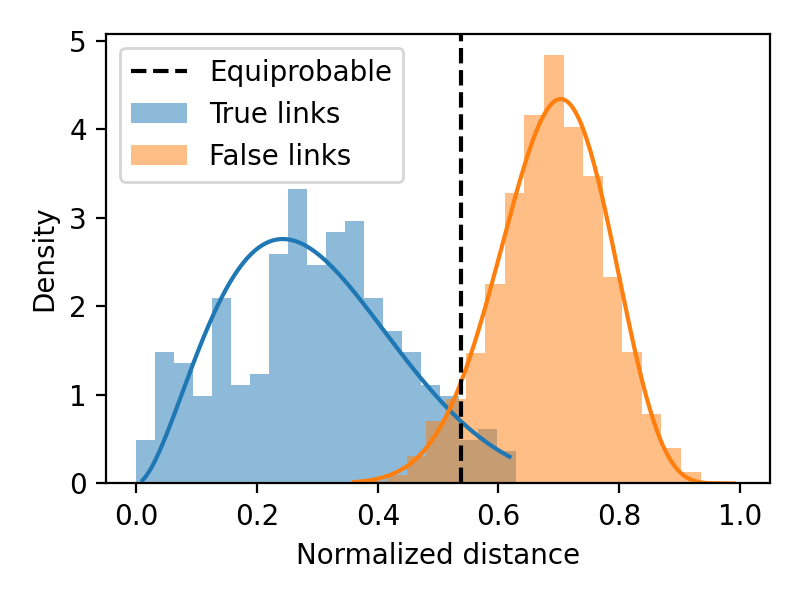
\includegraphics[width=\linewidth]{img/links_score_density.png}
\end{figure}

\subsubsection{Evaluation}

To evaluate the distribution-based clustering approach: Oxquarry, Brunet, St-Jean A and B are used.
Each retained rank list for each corpus is computed, see Table~\ref{tab:rls_oxquarry_brunet}~and~\ref{tab:rls_st_jean} in annex.
For each rank list, the distance threshold is computed, using the two beta approach.
This step corresponds to the training phase.
Then for every distance threshold and rank list pair, the clustering is evaluated using the $B^3_{F_1}$ and the $r_{diff}$.
This corresponds to the testing phase.

The evaluation results are aggregated by applying the arithmetic mean on the $B^3_{F_1}$ and $r_{diff}$ across all retained rank list.

The evaluation is presented in Table~\ref{tab:semi_supervised_clustering} show the results for each linkage criterion (Single, Average, Complete).

The following conclusions can be drawn with these results:
\begin{itemize}
  \item
  In terms of linkage criteria, the single linkage is not adapted with an average $B^3_{F_1} = 0.22$.
  Average linkage have the best $r_{diff} = 0.06$ which indicate that this criterion can estimate the most accurately the number of clusters.
  Complete linkage have the best $B^3_{F_1} = 0.82$ which make it the best criterion for this method.
  \item
  The training corpus does not influence a lot the quality of the results ($std(B^3_{F_1}) = 0.01$).
  The best corpus to train is Brunet, with slightly better results.
  \item
  In the other hand, the quality of the rank list used for the testing phase is more impactful ($std(B^3_{F_1}) = 0.04$).
  St-Jean B have the best rank list average precision and the best clustering results.
\end{itemize}

\begin{table*}
  \centering
  \caption{Distribution-based clustering evaluation, Mean retained rank lists $B^{3}_{F_1}$/$r_{diff}$ for each corpus pair}
  \label{tab:semi_supervised_clustering}

  \subcaption{Single Linkage}
  \begin{tabular}{l l| c c c c|c}
    \toprule
    \multicolumn{2}{c}{\multirow{2}{*}{}} & \multicolumn{4}{c}{Testing} \\
    \multicolumn{2}{c}{} & Oxquarry & Brunet & St-Jean A & St-Jean B & Mean \\
    \midrule
    \parbox[t]{2mm}{\multirow{4}{*}{\rotatebox[origin=c]{90}{Training}}}
    & Oxquarry  & 0.27/0.15 & 0.18/0.22 & 0.14/0.16 & 0.12/0.18 & 0.18/0.18\\
    & Brunet    & 0.36/0.12 & 0.18/0.22 & 0.15/0.16 & 0.12/0.18 & 0.20/0.17\\
    & St-Jean A & 0.42/0.11 & 0.30/0.19 & 0.14/0.16 & 0.13/0.18 & 0.25/0.16\\
    & St-Jean B & 0.42/0.10 & 0.35/0.16 & 0.16/0.16 & 0.16/0.17 & 0.27/0.15\\
    \midrule
    & Mean      & 0.37/0.12 & 0.25/0.20 & 0.15/0.16 & 0.13/0.18 & 0.22/0.16\\
    \bottomrule
  \end{tabular}

  \vspace{0.5cm}

  \subcaption{Average Linkage}
  \begin{tabular}{l l| c c c c|c}
    \toprule
    \multicolumn{2}{c}{\multirow{2}{*}{}} & \multicolumn{4}{c}{Testing} \\
    \multicolumn{2}{c}{} & Oxquarry & Brunet & St-Jean A & St-Jean B & Mean \\
    \midrule
    \parbox[t]{2mm}{\multirow{4}{*}{\rotatebox[origin=c]{90}{Training}}}
    & Oxquarry  & 0.73/0.04 & 0.65/0.08 & 0.59/0.10 & 0.61/0.11 & 0.65/0.08 \\
    & Brunet    & 0.78/0.05 & 0.73/0.04 & 0.73/0.07 & 0.73/0.08 & 0.74/0.06 \\
    & St-Jean A & 0.82/0.05 & 0.74/0.06 & 0.81/0.04 & 0.83/0.05 & 0.80/0.05 \\
    & St-Jean B & 0.83/0.09 & 0.79/0.08 & 0.83/0.02 & 0.90/0.02 & 0.84/0.05 \\
    \midrule
    & Mean      & 0.79/0.06 & 0.73/0.06 & 0.74/0.06 & 0.77/0.06 & 0.76/0.06 \\
    \bottomrule
  \end{tabular}

  \vspace{0.5cm}

  \subcaption{Complete Linkage}
  \begin{tabular}{l l| c c c c|c}
    \toprule
    \multicolumn{2}{c}{\multirow{2}{*}{}} & \multicolumn{4}{c}{Testing} \\
    \multicolumn{2}{c}{} & Oxquarry & Brunet & St-Jean A & St-Jean B & Mean \\
    \midrule
    \parbox[t]{2mm}{\multirow{4}{*}{\rotatebox[origin=c]{90}{Training}}}
    & Oxquarry  & 0.79/0.06 & 0.77/0.05 & 0.82/0.04 & 0.84/0.04 & 0.81/0.05 \\
    & Brunet    & 0.79/0.10 & 0.81/0.09 & 0.84/0.02 & 0.90/0.02 & 0.83/0.06 \\
    & St-Jean A & 0.79/0.11 & 0.81/0.11 & 0.82/0.05 & 0.90/0.02 & 0.83/0.07 \\
    & St-Jean B & 0.78/0.13 & 0.79/0.14 & 0.77/0.09 & 0.90/0.04 & 0.81/0.10 \\
    \midrule
    & Mean      & 0.79/0.10 & 0.80/0.10 & 0.81/0.05 & 0.88/0.03 & 0.82/0.07 \\
    \bottomrule
  \end{tabular}

\end{table*}
